\documentclass[12pt,openany]{book}

% Layout and fonts (pdflatex-safe)
\usepackage[T1]{fontenc}
\usepackage[utf8]{inputenc}
\usepackage{lmodern} % modern font family for pdflatex

\usepackage[paperwidth=8.5in,paperheight=11in,margin=0.6in]{geometry}
\usepackage{microtype}
\usepackage{setspace}
\usepackage{parskip}
\usepackage{ragged2e}
\usepackage{titlesec}
\usepackage{graphicx}
\usepackage{caption}
\usepackage{xcolor}

% --- Styling for children's book ---
\renewcommand{\familydefault}{\sfdefault} % use sans-serif
\setlength{\parindent}{0pt}
\titleformat{\chapter}[display]
  {\normalfont\Huge\bfseries\centering}
  {\chaptername\ \thechapter}{20pt}{\Huge}

% Big, friendly text for story
\newcommand{\bigpara}{\fontsize{18}{24}\selectfont}
\newcommand{\captionstyle}{\fontsize{12}{14}\selectfont\itshape}

% Helper for full-page image
\newcommand{\fullpageimage}[2][]{%
  \thispagestyle{empty}%
  \vspace*{0pt}%
  \begin{center}%
    \includegraphics[width=\paperwidth,height=\paperheight,keepaspectratio,#1]{#2}%
  \end{center}%
  \clearpage
}

% Helper for two-page spread
\newcommand{\twospread}[3][]{%
  \thispagestyle{empty}%
  \begin{figure}[!p]\centering
    \includegraphics[width=0.49\paperwidth,height=0.95\paperheight,keepaspectratio,#1]{#2}%
    \hfill
    \includegraphics[width=0.49\paperwidth,height=0.95\paperheight,keepaspectratio,#1]{#3}%
  \end{figure}
  \clearpage
}

\definecolor{accent}{HTML}{FF6F61}

\title{\Huge The Duck King of Lala}
\author{\Large By Your Name}
\date{}

\begin{document}
\frontmatter

% --- Title page ---
\begin{titlepage}
  \centering
  \vspace*{2cm}
  {\fontsize{36}{44}\selectfont\color{accent}\textbf{The Duck King of Lala}\par}
  \vspace{1.5cm}
  {\Large\textsc{A short tale for curious children}\par}
  \vfill
  {\Large By Your Name\par}
  \vspace{1cm}
  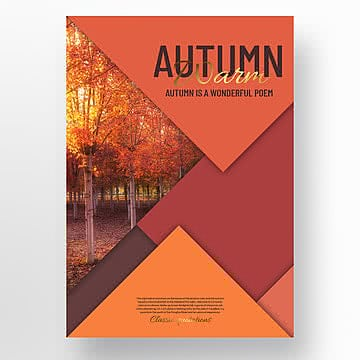
\includegraphics[width=0.5\textwidth]{images/sample_cover_illustration.jpg}
  \vfill
  {\small Copyright © \the\year\par}
\end{titlepage}

\cleardoublepage

% --- Dedication ---
\begin{center}
  \vspace*{3cm}
  {\large\itshape For little readers everywhere\par}
\end{center}
\clearpage

\tableofcontents
\clearpage

\mainmatter

% --- Chapter 1 ---
\chapter*{Chapter 1: The Duck King}
\addcontentsline{toc}{chapter}{Chapter 1: The Duck King}
\thispagestyle{empty}

\bigpara
\begin{flushleft}
Once upon a time in the pond of Lala, the Duck King woke up to a shiny, curious morning. 
He put on his small crown, which wobbled every time he smiled.\\[1em]

The Duck King loved feeding fireflies to his friends and telling tiny, funny stories about clouds that looked like jellybeans.
\end{flushleft}

\vspace{1.5cm}
\begin{center}
  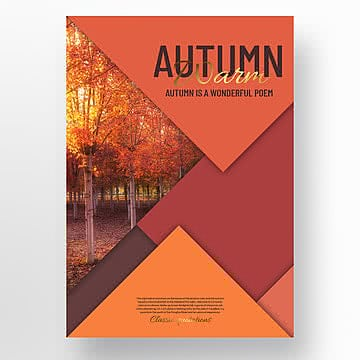
\includegraphics[width=0.8\textwidth]{images/duckking_small.jpg}
  \captionof{figure}{The Duck King and his crown.}
\end{center}

\clearpage

% --- Full-page image ---
\fullpageimage{images/spread_duck_king.jpg}

% --- Two-page spread ---
\twospread{images/left_page_scene.jpg}{images/right_page_scene.jpg}

% --- Chapter 2 ---
\chapter*{Chapter 2: Penny the Chicken}
\addcontentsline{toc}{chapter}{Chapter 2: Penny the Chicken}

\bigpara
Penny the chicken had a very loud giggle. She clucked songs that made the pond do silly dances. 
One morning, a small problem arrived — a lost kite tangled in the willow tree. Penny decided to help.
\vspace{1cm}

\begin{center}
  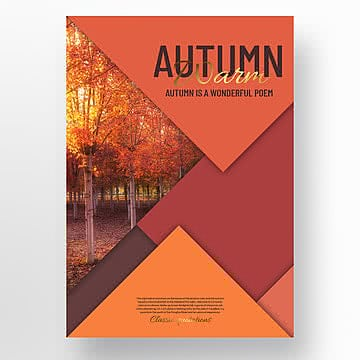
\includegraphics[width=0.6\textwidth]{images/penny.jpg}
  \captionof{figure}{Penny and the tangled kite.}
\end{center}

\clearpage

% --- Back matter ---
\backmatter
\chapter*{About the Author}
\addcontentsline{toc}{chapter}{About the Author}
\bigpara
Your Name loves telling stories, making silly drawings, and having tea with stuffed animals.

\clearpage

\chapter*{Acknowledgements}
\addcontentsline{toc}{chapter}{Acknowledgements}
\bigpara
Thanks to everyone who helped test the giggle-inducing lines.

\end{document}
